\section{Aufbau und Durchführung} % (fold)
\label{sec:durchfhrung}
\begin{figure}[h]
	\label{fig:drillachse}
	\centering
	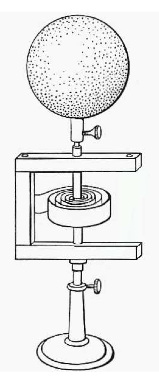
\includegraphics[height=7cm]{drillachse}
	\caption{Skizze des Versuchsaufbaus mit Kugel als Probekörper}
\end{figure}
In diesem Versuch wird die gezeigte Apparatur verwendet. 
Eine drehbar gelagerte Achse ist über eine Spiralfeder an einen festen Rahmen gebunden. 
In das obere Ende der Drillachse können verschiedene Körper eingespannt und der Auslenkwinkel $\phi$ anhand einer Skala abgelesen werden.
\subsection{Bestimmung der Winkelrichtgröße $D$}
\label{subsec:winkelricht}
Zur Bestimmung der Winkelrichtgröße $D$ wird gemäß \eqref{eq:Moment_Winkelricht} das Drehmoment $\vec{M}$ und der Auslenkwinkel $\phi$ ermittelt. Hierzu wird eine Metallstange so in die Vorrichtung eingespannt, 
dass die Drehachse durch den Stangenschwerpunkt verläuft senkrecht zur Drehachse steht.
Eine im Abstand $r$ zum Drehzentrum angehängte Federwaage misst die Kraft $F$ ausgehend vom rücktreibenden Drehmomentes bei Auslenkung der Metallstange um einen ausgewählten Winkel $\phi$. 
Zu beachten ist, dass die Federwaage senkrecht zum Stab und zur Rotationsachse sein muss. 
Dadurch kann der Betrag des Drehmoments $M$ durch
\begin{equation}
	| \vec{M} | = | \vec{r} \times \vec{F} | = |\vec{r}| |\vec{F}| \sin (\angle({\vec{r}})
\end{equation}
berechnet werden.
Diese Messung wird für 10 verschiedene Winkel $\phi$ zwischen 0 und $2\mathup{\pi}$ durchgeführt. 

\subsection{Bestimmung des Eigenträgheitsmomentes $I_{\mathup{D}}$ der Drillachse}
Auf die Metallstange aus Kapitel \ref{subsec:winkelricht} wird beidseitig im Abstand $a$ von der Drehachse je eine Masse befestigt.
Die Stange wird um $\phi$ ausgelenkt und mittels einer Stoppuhr die Schwingungsdauer $T$ für 2 Perioden gemessen. 
Es wird ein neuer Abstand $a$ gewählt und das Verfahren wiederholt, sodass insgesamt 10 Messwerte für Schwingungsdauer $T$ aufgenommen werden.
Masse und Abmessungen der Massestücke werden mit Waage und Schieblehre bestimmt.

\subsection{Bestimmung der Trägheitsmomente $I$ verschiedener Körper}
\label{subsec:traegheitkoerper}
Als erster Körper wird ein Styroporzylinder gewählt, welcher senkrecht auf die Drillachse gesteckt wird.
Anschließend wird der Körper in Schwingung versetzt und die Schwingungsdauer $T$ für 5 Schwingungen insgesamt 10 Mal gemessen. 
Das Verfahren wird für den zweiten Körper, eine Kugel, analog wiederholt.
Abmessungen und Masse der Probekörper werden mittels Schieblehre und Waage bestimmt.

\subsection{Bestimmung der Trägheitsmomente $I$ der Modellpuppe für zwei verschiedene Positionen}
\begin{figure}[h]
	\centering
	\label{fig:puppe}
	\begin{subfigure}{0.48\textwidth}
		\label{fig:puppe1}
		\centering
		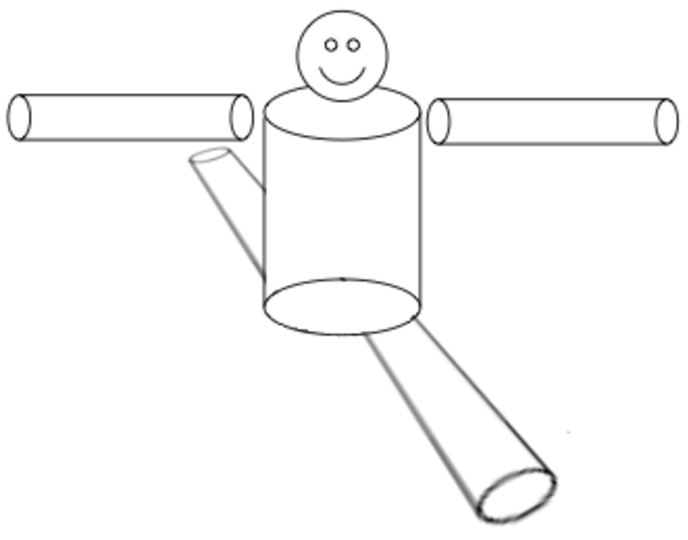
\includegraphics[width=5cm]{puppe1.pdf}
		\caption{Position (1) der Modellpuppe}
	\end{subfigure}
	\begin{subfigure}{0.48\textwidth}
		\label{fig:puppe2}
		\centering
		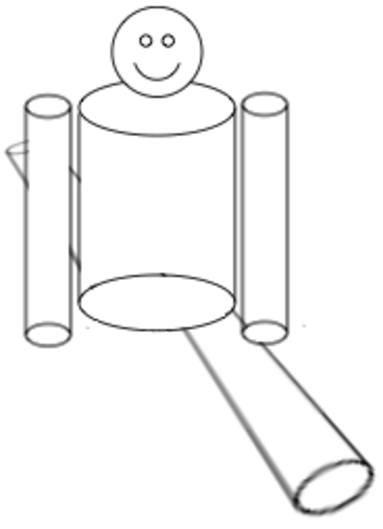
\includegraphics[width=3cm]{puppe2.pdf}
		\caption{Position (2) der Modellpuppe}
	\end{subfigure}
\end{figure}
Die Puppe wird jeweils in Position (1) und in Position (2)  in die Messvorrichtung eingespannt und 
der Messvorgang analog zu Kapitel \ref{subsec:traegheitkoerper} durchgeführt. 
Es folgen die Bestimmung des Gewichtes mit einer Waage und die Vermessung der einzelnen Körperteile der Puppe. 
Es werden Durchmesser und ggf. die Länge von Armen, Beinen, Kopf und Rumpf mit einer Schieblehre vermessen.

% section durchfhrung (end)
